%
% ISOTAS'96 paper
%
%           Author: Erick Gallesio [eg@unice.fr]
%    Creation date: 20-Jun-1995 11:54
% Last file update:  1-Dec-1995 14:57
%

\documentstyle[alltt,psfig]{llncs}
\begin{document}
% Command definitions
\newcommand{\figsize}{\small}
\newcommand{\stk}{\mbox{\sc STk}}
\newcommand{\stklos}{\mbox{\sc STklos}}
\newcommand{\Indextt}[1]{{\tt{#1}}\index{#1}}
\newcommand{\Index}[1]{{#1}\index{#1}}
\newcommand{\rrrr}{{\em R$^{4}\!RS$}}
\newcommand{\codesize}{\small}
\newenvironment{Code}{\begin{quote}\begin{minipage}{12cm}\codesize}{\end{minipage}\end{quote}}


\title{Designing a Meta Object Protocol to Wrap a Standard Graphical Toolkit}

\author{Erick Gallesio}
\institute {Universit\'e de Nice~~-~~Sophia~Antipolis \\
I3S/CNRS -  ESSI\\
Route des Colles - B.P. 145\\
06903 Sophia-Antipolis Cedex - FRANCE\\
Email: eg@unice.fr}

\maketitle


\begin{abstract}
This paper presents a graphical package which relies on the Tk toolkit and
the Scheme programming language. The Tk package is a widely used graphical
toolkit built upon the Tcl scripting language. Tcl was not designed as a
general purpose programming language and its usage for large-scale software
development is generally not suitable. To improve the programming level of
the Tk toolkit, we have defined {\stklos}, a Scheme language with a
CLOS-like object system. This alternative language has been used to embody
the standard Tk widgets in a clean hierarchy of classes, which is presented
here. The {\stklos} object system implementation is based on a Meta Object
Protocol; this protocol and its usage for accessing the Tk toolkit in an
efficient way are also presented here.
\end{abstract}


\section{Motivations}

The Tk package \cite{Ouster-book} is a widely used graphical toolkit which
provides a large set of widgets such as buttons, scrollbars, menus or text
editors. With these high level widgets, one can build rather complex
interfaces with little effort and without coping with the usual intricacies
needed when programming under the X window system {\cite{X11}}. The Tk
toolkit relies on a small interpretative scripting language named Tcl (Tool
Command Language)~\cite{Ouster-Tcl}, a string based language with a
shell-like syntax.

Tcl is a small scripting language. To easily embed the Tcl interpreter
in application programs, some usual programming languages capabilities
have been set aside by its author. In particular, Tcl has a poor set
of data structures reduced to character strings and associative
arrays. It provides numbers, which are simulated with strings and
which are, consequently, slow. In fact, a proper usage of Tcl consists
in writing small scripts to {\em glue} large application components
written in C or C++. However, experience shows that people are
reluctant to use it in this way, and that they often prefer to write
applications with a single programming language.

Tk is indeed an application with an embedded Tcl
interpreter~\cite{Ouster-Tk}. The interpretative nature of Tcl
provides Tk a simple and attractive interface to develop simple
graphical programs. However, the easiness afforded by Tcl for the
design of small interfaces is misleading and it often encourages
people to start heavy developments with this language. But, writing
large applications with a language which lacks ways of structuring
data tends to be more and more painful as the program grows. We think
that this kind of usage is beyond the scope of a language such as Tcl,
and we have tried to propose a solution for a better using of the 
Tk toolkit. 

In order to improve the Tk toolkit for large applications, we decided
to replace Tcl by a conventional programming language. Furthermore,
the {\em substitute} language must fulfill some important
requirements; it must be
\begin{itemize}
\item {\bf high level} and provides useful data types such as 
structures, arrays, lists or strings 
\item {\bf small} enough for allowing to embed it in
applications (as Tcl) 
\item {\bf efficient} so that most applications can be written
entirely in this language without having to resort to C or C++ programming.
\item easily {\bf extensible} so that user can investigate several
interesting programming paradigms ({\em e.g.} objects, prototypes,
actors,~\ldots)
\item already {\bf defined}. This point is, of course, not mandatory, but we
think that it is preferable to use an existing programming language, if
possible, rather than defining a new one.
\end{itemize}
Scheme \cite{R4RS} is a Lisp dialect which satisfies quite well the
previous points. It is a statically scoped language with a clear and
simple semantic. Moreover, Scheme procedures are first class objects
able to capture their creation environment. This language feature is
important since it allows us to envision the coding of interfaces {\em
callbacks} in a clean way. In this framework, we have defined
{\stk}~{\cite{Gallesio93-1}, a graphical package based on Tk toolkit
where the Tcl language as been replaced by a Scheme interpreter. 


{\stk} is a small and efficient Scheme interpreter.  As Tcl, it is
small enough to be used simply as a {\em glue language} which can be
embedded in an existing application. Furthermore, the solid basis
provided by the Scheme language affords the tools necessary for
writing, and maintaining medium size Graphical User Interfaces
(GUI). Nevertheless, we think the expressive power of Scheme is not
sufficient to envisage its use for large-scale software development.
In particular, the lack of an object mechanism increases the
programming complexity of large applications. {\stklos}, the object
extension of {\stk}, has been defined to alleviate this problem.  This
extension provides meta classes, multiple inheritance and generic
functions {\em \`a la} CLOS~\cite{CLOS,CLtL2} or Dylan~\cite{Dylan}.
{\stklos} has also been used to embody the predefined Tk widgets in a
hierarchy of classes. Usage of these classes simplifies the core Tk
usage by providing an homogeneous access to widget options and by
hiding the Tk widgets low level idiosyncrasies. Moreover, as expected,
usage of objects facilitates code reuse and definition of new widgets
classes. Finally, we think that the object orientation of {\stklos},
as well as the solid basis of the Scheme programming language, afford
therefore the tools necessary to envision writing, and maintaining,
complex GUI.


The rest of this paper is divided in three sections. The next section
presents the {\stk} package and its object system. Wrapping the
standard Tk widgets in {\stklos} classes and the influence of this
integration in interfaces programming are described in section 3.
{\stklos} implementation relies on a MOP (Meta Object Protocol), in
the spirit of the one defined for CLOS~\cite{AMOP}. Section 4 presents
this protocol and how it has been used to integrate the Tk standard
widgets in the Scheme world.


%%%%%%%%%%%%%%%%%%%%%%%%%%%%%%%%%%%%%%%%%%%%%%%%%%%%%%%%%%%%%%%%%%%%%%%%%%%%%%

\section{Presentation of {\stklos}}

Programming with {\stk} can be done at two distinct levels. The first
level uses only the standard Scheme constructs and is quite
classical. The second level gives access to {\stklos}, the object
oriented extension of {\stk}. Of course, both levels can be used at
the same time in a single program. However, most of the time, one will
use the higher level, resorting to the lower one for specific purposes
only.

\subsection{\stk: the Basic Layer}

Starting a session with {\stk} brings the user in the
basic layer which gives access to an extended Scheme interpreter
able to handle the Tk toolkit. With a little set of rewriting
rules from the original Tcl/Tk library, and the Tk manual pages close
at hand, one can easily build a {\stk} program using the Tk toolkit.

Creation of new widgets (button, label, canvas, \ldots) is done by
special {\stk} primitives procedures. For instance, creating a new
button can be done as followed
\begin{quote}\figsize
\begin{verbatim}
(button '.b)
\end{verbatim}
\end{quote}
Tk uses a very special way to name widgets: a widget name is a kind
of pathname which reflects its position in
the graphical hierarchy of widgets. In this example, the name of the
newly created button is ``{\tt .b}''. This pathname states that ``{\tt
b}'' is a son of ``{\tt .}'', the root window. Note that the name of
the widget must be {\em quoted} due to the Scheme evaluation
mechanism. 

Calling a widget creation primitive, such as {\tt button},
builds a new Scheme object which is called a {\em Tk-command}. This
object, which is considered as a new basic type by the {\stk}
interpreter, is automatically stored in a variable whose name is the
symbol given to the creation function ({\tt .b} in this case).  A
Tk-command is a special kind of function which is generally used, as
in Tcl/Tk, to customize its associated widget. For instance, the
expression\label{configure}
\begin{quote}\figsize
\begin{verbatim}
(.b 'configure :text "Hello, world" :border 3)
\end{verbatim}
\end{quote}
\noindent
allows us to set the text and background options of
the~{\tt .b} button. Of course, as in Tcl/Tk, parameters can be passed
at widget creation time, and the previous button creation and
initialization could have been done in a single expression, such as
\begin{quote}\figsize
\begin{verbatim}
(button '.b :text "Hello, world" :border 3)
\end{verbatim}
\end{quote}
\noindent

Tk proposes a general purpose binding mechanism to associate 
a handlers to an external event ({\em e.g.} a key press or a mouse
action). An event handler is automatically triggered by the library
when the given event occurs. In Tcl, an event handler is a string which is
evaluated at the global level, whereas in {\stk} it is a Scheme
closure. The following expression adds a new event handler to the {\tt
.b} button when the third mouse button is depressed over it:
\begin{quote}\figsize
\begin{verbatim}
(bind .b "<ButtonPress-3>"
      (let ((count 0))
        (lambda ()
          (set! count (+ count 1))
          (format #t "# of button press: ~A~%" count))))
\end{verbatim}
\end{quote}

This simple example shows that {\stk} handlers are cleaner than Tcl ones: 
the standard Scheme lexical scoping allows a handler to have its own
private global variables (as {\tt count} here); on the other hand, a Tcl
handler is a flat string unable to carry an environment.

Even if closures afford a better expressive power for writing event
handlers than Tcl strings, programming an interface resorting only to the
constructions of the basic layer becomes rapidly tedious. In fact, the
{\stk} basic layer can be considered as a kind of {\em assembly language}
for interfaces programming and we will see in section~\ref{reification} how
it can be used for the {\em reification} of the Tk widgets in {\stklos}
classes.

%%%%%%%%%%%%%%%%%%%%

\subsection{\stk: the Object Layer}

{\stklos}, the object extension of {\stk}, is close to the CLOS
system~\cite{CLOS}; it is briefly introduced in this section. Note that we
consider only the language aspects of {\stklos} here and we 
forget its use for integrating the Tk toolkit for a while.


Definition of a new class is done with the {\tt define-class} macro. For
instance, 
\begin{quote}\figsize
\begin{verbatim}
(define-class Point ()
   ((x :init-keyword :x :accessor x-of)
    (y :init-keyword :y :accessor y-of)))
\end{verbatim}
\end{quote}
defines the characteristics of a point. Two slots are declared here: {\tt
x} and {\tt y}.
\noindent
Creation of new instances is done with the {\tt make} constructor: 
\begin{quote}\figsize
\begin{verbatim}
(define p (make Point :x 10 :y 20))
\end{verbatim}
\end{quote}
\noindent
The evaluation of the preceding form builds a new point and initializes
its slots {\tt x} and {\tt y} with the values 10 and 20. Slot content
can be accessed by the two basic primitives {\tt slot-ref} and {\tt
slot-set!}. These primitives are low level primitives and users often
prefer to use accessors, since they generally lead to a clearer
code. For instance, getting the value of the {\tt y} slot of {\tt
p} could be done in the following way:
\begin{quote}\figsize
\begin{alltt}
(y-of p)                {\em ; or (slot-ref p 'y)}
\end{alltt}
\end{quote}
\noindent
since the {\tt y-of} accessor has been defined for slot {\tt
y}. This slot can be set by the generalized {\tt set!}\label{set!}
form, as illustrated by the following example:
\begin{quote}\figsize
\begin{alltt}
(set! (y-of p) 1)       {\em ; or (slot-set! p 'y 1)}
\end{alltt}
\end{quote}

\noindent
Now, we can define the {\tt Rectangle} class which inherits from the {\tt
Point} class: 
\begin{quote}\figsize
\begin{verbatim}
(define-class Rectangle (Point)
  ((width  :init-keyword :width  :accessor width-of)
   (height :init-keyword :height :accessor height-of)))
\end{verbatim}
\end{quote}
\noindent
The instances of this class have four slots ({\tt x}, {\tt y}, {\tt width}
and {\tt height}).  Methods\footnote{In {\stklos}\cite{Gallesio95-1a}, the
execution of a method rely on a subset of the CLOS {\em generic functions}
mechanism (only primary methods are supported and the methods combination
cannot be changed).}  defined for instances of the {\tt Point} class can
also be used for instances of the {\tt Rectangle} class. For example, the
{\tt x} coordinate of a {\tt Rectangle} can be accessed with the accessor
method {\tt x-of} defined before.


Previous class definition represents rectangles with a reference point, a
width and a height. This representation for rectangles is, most of the
time, convenient but we sometimes need a representation using the
coordinates of two opposite corners. In that case, {\em virtual slots} can
be used\label{virtual-slot}. A virtual slot is a slot which is defined as a
normal slot but whose allocation is declared as {\tt :virtual}. Such a slot
has a null allocation and its reading (resp. writing) provokes the
execution of a getter (resp. setter) function which must be provided by the
user within the class definition. The getter and setter functions are
defined with the {\tt :slot-ref} and {\tt :slot-set!} options. Here is
another writing of the {\tt Rectangle} class using virtual slots:

\begin{quote}\figsize
%\begin{minipage}{12.2cm}
\begin{alltt}
(define-class Rectangle (Point)
  ((width  :init-keyword :width  :accessor width-of)
   (height :init-keyword :height :accessor height-of)
\end{alltt}
%\end{minipage}
%\begin{minipage}{12.2cm}
\begin{alltt}
   (x2     :init-keyword :x2     :accessor x2-of 
           :allocation   :virtual
           :slot-ref  (lambda (obj) (+ (x-of obj) (width-of obj)))
           :slot-set! (lambda (obj val) 
                        (set! (width-of obj) (- val (x-of obj)))))
\end{alltt}
%\end{minipage}
%\begin{minipage}{12.2cm}
\begin{alltt}
   (y2     :init-keyword :y2 :accessor y2-of 
           :allocation   :virtual
           :slot-ref  (lambda (obj) (+ (y-of obj) (height-of obj)))
           :slot-set! (lambda (obj val) 
                        (set! (height-of obj) (- val (y-of obj)))))))
\end{alltt}
%\end{minipage}
\end{quote}
In this new definition of {\tt Rectangle}, {\tt x2} and {\tt y2} are
virtual slots. The getter and setter associated functions are
lambda expressions which  compute or set their value depending on
other slots value. Note that a  virtual slot accessor closure can
change the value of standard slots in order to keep the system
coherent.

Since virtual slots do not imply memory allocation, they could easily be
simulated with classical accessor methods. But, declaring a slot as
virtual allows introspecting functions to ``see'' it as a standard slot. On
the contrary, using a couple of methods to simulate such a slot would hide
it to these functions.

%%%%%%%%%%%%%%%%%%%%%%%%%%%%%%%%%%%%%%%%%%%%%%%%%%%%%%%%%%%%%%%%%%%%%%%%%%%%%%

\section{Integration of Tk widgets}
\label{reification}

\subsection{The Class Hierarchy}

This section presents how the standard Tk widgets have been embodied in
{\stklos} classes. Each graphical object defined in the Tk toolkit such as
menu, label or button is represented by a {\stklos} class. The
corresponding classes constitute a hierarchy which is briefly described
here. First, all the classes share a unique ancestor: the {\tt <Tk-object>}
class\footnote{End users will not have to use direct instances of the {\tt
<Tk-object>} class (all classes whose name begins with the ``Tk-'' prefix
are abstract classes which should not be instanced; they correspond to the
{\em implementation specific} classes of
\cite{Kickzales:oopsla92}).}. This class defines a set of slots
necessary to establish a communication between the Scheme and Tk
worlds. In particular, two slots are defined in this
class\footnote{The actual implementation is more complex, but to make
easier the reading of this paper, we have simplified the definition of
classes, and hence the class hierarchy.}:
\begin{itemize}
		\item The {\tt parent}\label{parent-slot} slot contains a
reference to the object which (graphically) includes the current object.
\item The {\tt Id} slot contains a reference to the low level {\stk} {\em
Tk-command} which implements the {\stklos} widget. This {\em Tk-command},
which is different for each class, is created during {\stklos} instance
initialization. This slot establishes the link between the {\stk} and the
{\stklos} layers and guarantees, by keeping a reference to the low level
widget, a protection against GC recovery.
\end{itemize}

The next level of the class hierarchy defines a fork with two
branches: the {\tt <Tk-widget>} class and {\tt <Tk-canvas-item>}
class. Instances of the former class are classical widgets such as
buttons or menus whereas instances of the later are objects contained
in a canvas\footnote{The canvas widget afforded by the Tk library
allows 2D structured drawing.} such as lines, ovals or
rectangles. Both kind of Tk objects are directly implemented as
{\stklos} classes in a one-to-one relationship. A partial view of the
{\stklos} hierarchy is shown in Fig.~1. Here are some important
points:
\begin{figure}
%\centerline{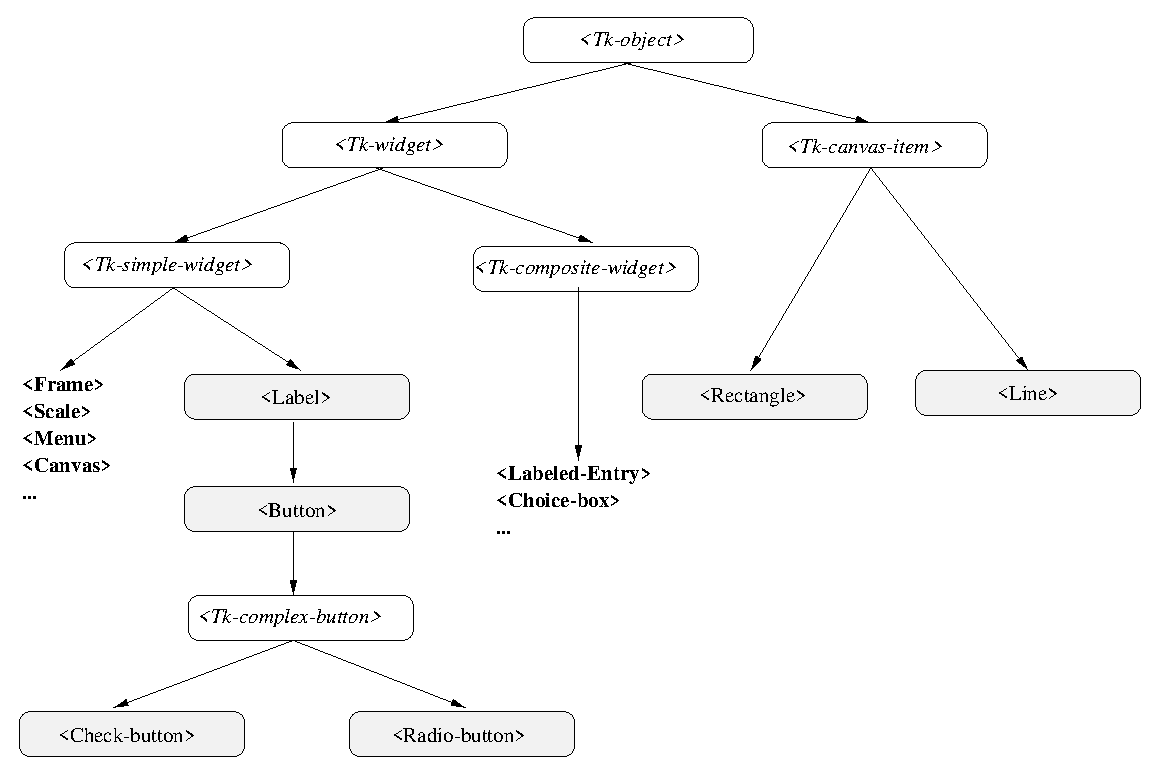
\epsfig{file= hierarchy.eps, clip=, width=13cm,height=13cm}}
\centerline{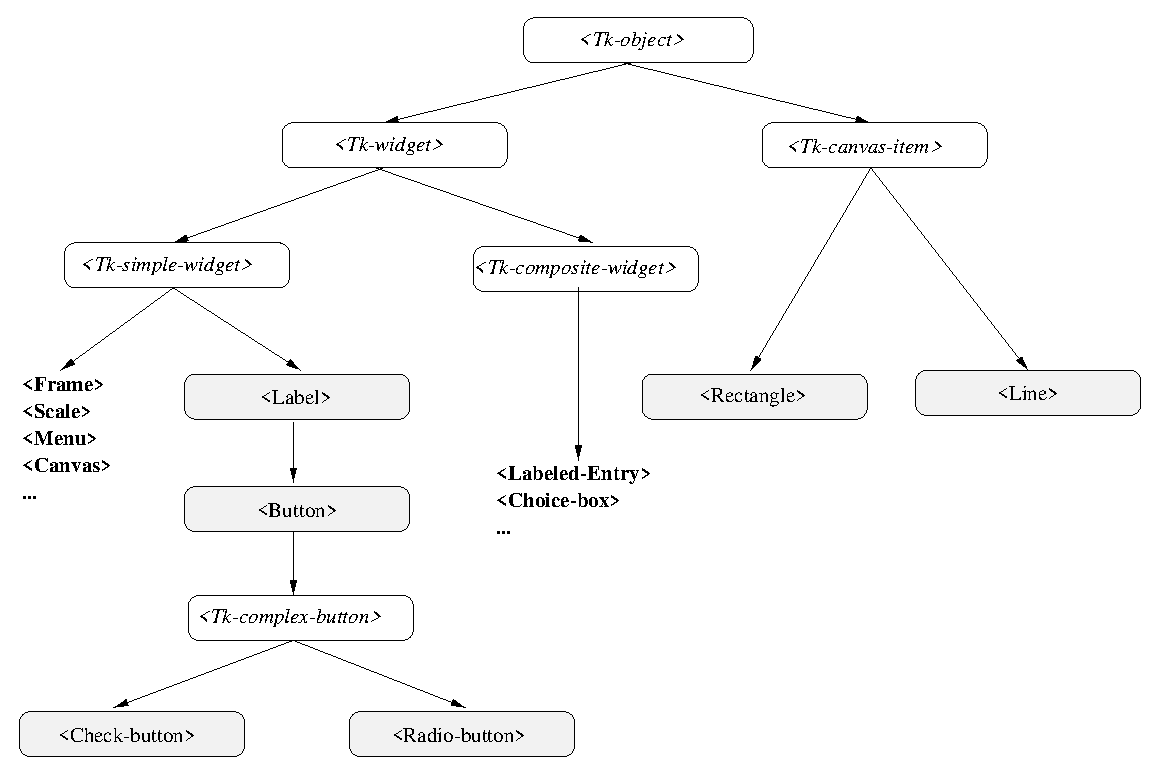
\psfig{file= hierarchy.eps,width=12.0cm}}
\caption[]{\em A partial view of the {\stklos} hierarchy}
\end{figure}
\begin{itemize}
		\item In Tk, interface widgets ({\em e.g.} buttons) are
first class objects, but canvas items ({\em e.g.} rectangles) can be
accessed only through their containing canvas. Thus, actions on widgets or
canvas items must be done in different ways.  Accessing a canvas item
option requires two references: one to the canvas which contains it and one
to its identification (a number) in this canvas. In order to make canvas
items first class objects, the class {\tt <Tk-canvas-item>} defines the
extra slot {\tt Cid} which contains the Tk identification number associated
to the item.

		\item The hierarchical view of Tk widgets permits a better
apprehension of the Tk toolkit, even if there is no notion of inheritance
in standard Tk. According to Fig.~1, a {\em button} can be seen as a
reactive {\em label}. As a consequence, the methods in charge of the look
of a label or button text (font, foreground color, \ldots) can be gathered
in the {\tt <Label>} class. Thus, the {\tt <Button>} class has only to
manage the operations which are specific to a reactive text, such as the
associated command to invoke when the mouse button is depressed over it.

		\item Simple and composite widgets share a common
ancestor ({\tt <Tk-widget>}). Consequently, composites widgets, which
are written in Scheme, are controlled exactly in the same way as C
built-in Tk widgets. This kind of widgets is discussed in~\cite{Gallesio94-1}.
\end{itemize}

\subsection{Accessing Tk Widgets Options}

Each Tk toolkit widget accepts a specific set of options which enables its
aspect customization such as its color, font, text or relief. Options may
be specified either on the command line when the widget is created or with
the {\tt configure} operation which is applicable to all Tk widgets. In
{\stklos}, each option of a Tk widget is seen as an object slot, and
getting or setting the configuration of a Tk option is equivalent to read
or write an object slot. The following example shows a possible {\stklos}
definition of a Tk button.

\begin{quote}\figsize
\begin{minipage}{12cm}
\begin{verbatim}
(define-class <Button> (<Label>)
   ((command :accessor command :init-keyword :command 
             :allocation :tk-virtual))
   :metaclass <Tk-metaclass>)
\end{verbatim}
\end{minipage}
\end{quote}
This new class inherits from {\tt <Label>} and owns an extra slot
called {\tt command}.  The allocation of this slot is qualified with
{\tt :tk-virtual}. \label{tk-virtual}Tk-virtual slots are special
purpose slots: they can be used as normal slots but they are not
allocated in the Scheme world ({\em i.e.} their value is stored in one
of the structures manipulated by the Tk library instead of in a Scheme
object). Consequently, reading or writing such a slot is done in a
particular way: access to Tk-virtual slot uses in turn the standard Tk
{\tt configure} operation as in \ref{configure}. Tk-virtual widgets
slots are a special kind of virtual slots which are managed by the
meta class {\tt <Tk-metaclass>}. Defining a class using this meta
class allows the modification of a slot accessors at the lowest
level. Therefore, the value of a virtual slot always reflect the
actual value of the associated Tk option (remember that no space is
reserved for this slot in the Scheme core and that accesses are
directly done within the Tk data structures). The specification of the
meta class of the {\tt <Button>} class in given with the {\tt
:metaclass} option\footnote{In fact, this meta class citation can be
omitted since {\tt <Label>} (or one of its ancestor) has probably
already specified it. In this case the system will automatically
choose the most specific meta class.}.  It is important to note that
the construction of the slot accessors is made at class creation so
that no particular computation is necessary when accessing such a
slot. Thus, customizing a widget by using a slot access at the
{\stklos} level is {\bf as efficient as} using a standard Tk option
configuration at the {\stk} base level.

The previous definition of {\tt <Button>} is not sufficient for a
complete integration of the Tk button widget in a {\stklos} class. Indeed,
the MOP ensures that {\tt Tk-constructor}\label{Tk-constructor} is called
when creating a new {\tt <Tk-widget>} (and {\tt <Button>} is an indirect
instance of {\tt <Tk-widget>} as shown in Fig.~1). This function must
determine the Tk library function (a {\em Tk-command}) which has to be
called to create the new widget.  The following method for {\tt
Tk-constructor} suffices to do this job:
\begin{quote}\figsize
\begin{verbatim}
(define-method Tk-constructor ((b <Button>)) 
   button)
\end{verbatim}
\end{quote}
The previous {\tt <Button>} class and {\tt Tk-constructor} method
definitions are the two only things necessary for defining a new {\stklos}
widget. This point is particularly important since it permits to minimize
the integration cost of new Tk widgets and, consequently, to {\em follow}
future Tk releases with minimal coding.

The following variable definition shows how we can use the above 
{\tt <Button>} class:
\begin{quote}\figsize
\begin{verbatim}
(define b (make <Button> :font "fixed" 
                         :command (lambda () (display "Hello\n"))))
\end{verbatim}
\end{quote}

\noindent
This expression assigns to the symbol {\tt b} a new instance of 
{\tt <Button>}. Changing the font or the command associated to
this object could be done by using either the {\tt slot-set}! or the
generalized {\tt set}!  primitives as shown in~\ref{set!}.


\subsection{Comparison of {\stklos} and Standard Tk}

Some of the advantages of {\stklos}, approach over standard Tk have
already been discussed before. In this section, we go on further this
discussion.

\subsubsection{Low Level Detail Hiding}

One of the most important benefits when embodying Tk widgets in {\stklos}
is that most of the Tk idiosyncrasies are hidden to the user. As a positive
consequence, this improves greatly the level we can program GUI. A
major improvement concerning this point is that we do not need anymore to
take care of the Tk widget naming conventions. The fact that Tk imposes
that the name of a widget must reflect the hierarchy to which it belongs,
and the lack of relative naming conventions are very severe constraints
when designing a GUI. These points make difficult, in standard Tk, the
definition of reusable interface components and usage of long pathnames
(which are current in non toy applications) is very awkward to
manage. Furthermore, these conventions lead to change large pieces of code
as soon as a modification is done in the widget hierarchy. In this sense,
Tk naming conventions do not fit well with GUI programming since the design
of an interface brings aesthetic problems which often conduct to develop it
on a trial and error basis.

In {\stklos}, Tk naming convention are completely hidden and the only
thing the user needs to know when creating a new object is the widget
which contains it. This object is called its parent. An example of
nested widgets creation is shown below:

\begin{quote}\figsize
\begin{verbatim}
(define f  (make <Frame>))
(define b1 (make <Button> :text "B1" :parent f))
(define b2 (make <Button> :text "B2" :parent f))
\end{verbatim}
\end{quote}

\noindent
The buttons {\tt b1} and {\tt b2} created here specify that their parent
is the frame {\tt f}. Since this frame does not specify a particular
parent, it is supposed to be a direct descendant of the root
window. Note that only the definition of {\tt f} should be changed if
we decide that {\tt f} should no more be a top-level frame. A
modification in the hierarchy of this widget is automatically
propagated to all the widgets belonging to this hierarchy.  {\stklos}
also extends this parent notion to take into account canvas items
(rectangles, lines, ovals,~\ldots): a canvas item is considered to be
a descendant of the canvas which contains it. This vision of the
canvas items allows the {\stklos} user to manipulate canvas items as
first class objects. For instance,

\begin{quote}\figsize
\begin{verbatim}
(define c (make <Canvas>))
(define r (make <Rectangle> :parent c :coords '(0 0 50 50)))
\end{verbatim}
\end{quote}


\noindent
defines a rectangle called {\tt r} in the {\tt c} canvas. As said
before, accessing this rectangle implies the use of two references in
standard Tk: the canvas which contains it, and its identification
number in this canvas. In {\stklos}, both informations are contained in the object
which represent the rectangle. For instance, after executing the expression,
\begin{quote}\figsize
\begin{verbatim}
(bind r "<Enter>" (lambda (x y) 
                     (format #t "Mouse enters in ~A ~A~%" x y)))
\end{verbatim}
\end{quote}

\noindent
a message is displayed, each times the mouse enters the {\tt r}
rectangle. It is important to note here that we would use {\em
exactly} the same expression to associate such a binding to a simple
widget such as a button or a label, whereas it needs two different
syntactic forms in Tcl/Tk, since the procedures which access
a canvas item or an interface widget are different.

\subsubsection{Uniform Access to the Toolkit}
Usage of generic functions is also a significant improvement over the
Tk basic level programming since it allows an homogeneous access to
Tk commands. Suppose that we want to give access to
the value of a {\tt scale} or an {\tt entry} widget with the generic
function {\tt value}. This can easily be done by the following method
in {\stklos}:

\begin{quote}\figsize
\begin{verbatim}
(define-method value ((obj <Tk-simple-widget>))
   ((Id obj) 'get))
\end{verbatim}
\end{quote}

In this case, one method is sufficient to implement the getter
function since the Tk sub-option for reading the value of a scale or
an entry is the same. Writing the setter function for those widgets is
a little bit more complicated since the way of changing a scale value
is different from the way of changing an entry value in Tk:

\begin{quote}\figsize
\begin{verbatim}
(define-method (setter value) ((obj <Scale>) v)
  ((Id obj) 'set v))

(define-method (setter value) ((obj <Entry>) v)
  ((Id obj) 'delete 0 'end)
  ((Id obj) 'insert 0 v))
\end{verbatim}
\end{quote}

Using the same generic function (with two different methods) permits to
hide to the user these low level details and gives him/her a coherent
access to the toolkit. In the call, {\label{value}}
\begin{quote}{\figsize
\begin{verbatim}
(set! (value x) 100)
\end{verbatim}
}\end{quote}
\noindent
the system chooses the method to apply depending on the class of {\tt
x}. Of course, an error\footnote{more exactly, the system calls the
{\tt no-applicable-method} generic function which, by default, signals
an error, as in CLOS. User can specialize this function to provide
another handler.} will be signaled if {\tt x} is not an
entry or a scale.  Note that this notion of widget value could also be
easily implemented with a virtual slot (see~\ref{virtual-slot}) even
if {\tt :value} does not exist as a Tk option {\it per~se}. This
approach, which is the one chosen in the current released library,
allows introspecting functions to manage the value of a widget as
a standard slot. In particular, this library offers a small interface
builder which heavily use introspection to automatically build
specialized widget editors. Defining {\tt value} as a virtual slots
for most widgets allows the user to tune it in the same fashion as the
font or the background Tk options. Designing an interface builder
using only standard Tk constructs would have been a lot more
painful.


The previous examples show that programming with {\stklos} brings the power
of a full featured object language in the area of GUI
construction. However, this fine integration of the Tk toolkit could not
have been done without the underlying Meta Object Protocol of
{\stklos}. This protocol is discussed in the following section.


\section{Implementation}

In the previous section, we show through several examples the gain provided
by an object language to use the Tk toolkit. The simplicity of these
examples could make think that the definition of an {\em ad-hoc} object
system for Tk widgets could suffice to have an OO vision of the
toolkit. However, we feel that this approach, which has been widely
used for Tcl, is not the good one. Providing a general purpose Scheme
object system, which can easily be customized for using Tk, seems a
far better approach.  Indeed, in the GUI area, applications
programmers often need to be able to use introspection on the objects
they manipulate, or they need to define new ways to access object
slots when composing several widgets. These constraints have led us to
define a MOP based object extension for {\stk}, because it is probably
the cleanest way to achieve the requirements expressed above.

This section presents how to integrate Tk widgets in a hierarchy such
as the one shown in Fig.~1. The discussion is split in two
parts. First, we present the services a MOP must offer for this
integration and then, we show how we can exploit them to build
this hierarchy.

\subsection{The {\stklos} Meta Object Protocol}

{\stklos} meta object protocol implementation is based on
Tiny-Clos~\cite{Tiny-Clos}, a minimal MOP written in Scheme. Current
version of {\stklos} MOP is written in C and in Scheme. Code written in C
correspond to the generic functions calls, which allows to implement them
as efficiently as possible.  The rest of the implementation, where time
consumption is less important ({\em e.g.}~computation of class
precedence lists or printing methods), is written in Scheme. This conducts
to an efficient implementation where the overhead of OO programming {\it
vs} ``classical'' programming is as low as possible.

As said before, {\stklos} is a general purpose OO extension, but a great
attention has been carried for the services its MOP must provide in order
to integrate easily and efficiently Tk widgets in {\stklos} objects. The
{\stklos} protocol must at least offer following capabilities:
\begin{itemize}
\item a way to  intervene in the initialization of a {\stklos} widget.
The first task which must be done at this stage consists to generate a
name (using the Tk conventions) for the widget which will implement
the new instance. Then, the instance creation arguments list must be
filtered to distinguish the user arguments which concern only
{\stklos} ({\em e.g.}~the {\tt parent} slot discussed in
\ref{parent-slot}) from those which correspond to Tk
options. This distinction among parameters is necessary because the Tk
library raises an error when it encounters a parameter it does not know
how to manage.

\item the possibility to define slots with special behaviour and
allocation schemes. In effect, beyond virtual slots already discussed
in \ref{virtual-slot}, the protocol should allow to map the Tk widget
options  as slots of a {\stklos} object. Note that the
way to do this mapping will be different for a simple widget and a
canvas item, since Tk offers two different methods for accessing their
options. Furthermore, the protocol for defining slots must be as
simple as possible to allow application programmers to extend the
library with new kinds of widgets.
\end{itemize}

The creation of a {\stklos} object is done with the {\tt make} generic
function. As in CLOS, this function first allocates a new instance
(by calling the generic function {\tt allocate-instance})
and then returns this instance initialized. Initialization of the
new instance is performed by the {\tt initialize} generic function. 

Class slots are computed when the class is initialized. The {\stklos}
MOP calls the generic function {\tt compute-get-n-set} which, given
the definition of a slot, returns a couple of procedures. These
procedures correspond to the reader and writer functions for the
slot. In case of a virtual slot definition (see~\ref{virtual-slot}),
for instance, {\tt compute-get-n-set} returns a list constituted of
the two evaluated lambda expressions given in the {\tt :slot-ref}
and {\tt :slot-set!} options.

\subsection{Using the MOP to Wrap Tk Widgets}

We present here only the salient points which are necessary to the
integration of Tk widgets and simple canvas items in an object
world. The code exposed here is simpler than the one which is used in
the current distribution of {\stk}, but principles are the same. A
complete listing of the source code of this simplified implementation
is given in annex.

\subsubsection{Managing Tk Options as Object Slots.} 

When a new class is created, the generic function {\tt
compute-get-n-set} is called for each slot this class defines. This
function takes two parameters: the class which is being created and
the slot definition (a list). This allows us to define a meta class
which takes into account a special kind of slots: {\em tk-virtual}
allocated slots. The meta class in charge of these slots is called
{\tt <Tk-metaclass>}. This class is defined as:
\begin{quote}\figsize
\begin{verbatim}
(define-class <Tk-metaclass> (<class>)
  ((valid-options :accessor Tk-valid-option)))
\end{verbatim}
\end{quote}
The slot {\tt valid-options} contains the list of options a Tk widget
recognizes. This slot is initialized when a new widget class is defined
(its value is set to the list of the slots whose allocation is {\em
Tk-virtual}). Usage of {\tt valid-options} will be discussed later.

Tk-virtual slots have been presented in~\ref{tk-virtual}. Reading and
writing this kind of slot implies the use of the {\tt configure} sub-option
which is always available for Tk widgets. In standard Tk, reading the value
of a widget option, such as {\tt width}, for a given widget {\tt w} must
be done with
\begin{quote}\figsize
\begin{verbatim}
(list-ref (w 'configure :width) 4)
\end{verbatim}
\end{quote}
\noindent
Setting the width of this widget to the value {\tt val} is a little
bit simpler and can be expressed as:
\begin{quote}\figsize
\begin{verbatim}
(w 'configure :width val)
\end{verbatim}
\end{quote}

\noindent
Consider now a canvas item whose enclosing canvas and identification number
are respectively {\tt c} and {\tt id}; reading and writing the value 
of its {\tt width} option can be done with 
\begin{quote}\figsize
\begin{verbatim}
(list-ref (c 'itemconfigure id :width) 4)
\end{verbatim}
\end{quote}
and
\begin{quote}\figsize
\begin{verbatim}
(c 'itemconfigure id :width val)
\end{verbatim}
\end{quote}

\noindent
We said in previous subsection that the generic function {\tt
compute-get-n-set} has in charge slot allocation.  Given the Tk conventions
exposed before, it is easy to define a {\tt <Tk-metaclass>} specialized
method for this function. This method must return a list whose first
element is a closure for reading the slot, and whose second element is a
closure for its writing:

\begin{quote}\figsize
\begin{alltt}
(define-method compute-get-n-set ((class <Tk-Metaclass>) slot)
  (if (eqv? (get-slot-allocation slot) :tk-virtual)
      {\em ;; this is a Tk-virtual slot}
      (let ((opt (make-keyword (car slot))))
        (list (lambda (obj) (list-ref ((Id obj) 'configure opt) 4))
              (lambda (obj val) ((Id obj) 'configure opt val))))
      {\em ;; call super compute-get-n-set}
      (next-method)))
\end{alltt}
\end{quote}

\noindent
This method first tests the allocation type of the slot with {\tt
get-slot-allocation}. If the slot is a Tk-virtual one, this method
returns the reader and writer closures in a list. Otherwise, this
method calls {\tt next-method}, that is to say the {\tt
compute-get-n-set} method defined over the super class of {\tt
<Tk-metaclass>}.

Since Tk accesses canvas items options in a different way than simple
widgets ones, {\tt <Tk-metaclass>} cannot be used for reading and
writing their slots. A meta class for canvas items can be simply
defined as
\begin{quote}\figsize
\begin{alltt}
(define-class <Tk-item-metaclass> (<Tk-Metaclass>)
  ())
\end{alltt}
\end{quote}
\noindent
Given this meta class and the Tk conventions shown before, it is simple to
define a {\tt compute-get-n-set} method specialized for canvas items:
\begin{quote}\figsize
\begin{alltt}
(define-method compute-get-n-set ((class <Tk-item-metaclass>) slot)
  (if (eqv? (get-slot-allocation slot) :tk-virtual)
      (let ((opt (make-keyword (car slot))))
        (list (lambda (obj)   
                (list-ref ((Id obj) 'itemconfigure (Cid obj) opt) 4))
              (lambda (obj val) 
                ((Id obj) 'itemconfigure (Cid obj) opt val))))
      (next-method)))
\end{alltt}
\end{quote}

\noindent
Two points are important to note here:
\begin{itemize}
\item  Methods of the generic function {\tt compute-get-n-set} are 
very dependent of the procedure Tk proposes for accessing widget
options. However, it must be noted that only the two returned lambda
expressions should be re-written if the author of the Tk toolkit
decides to change current conventions. We can even say that the MOP
permits to write programs which are less dependent of the Tk toolkit
than Tcl/Tk programs, since dependences can be isolated in a few
methods instead of being spread all over the code.
\item The protocol for accessing the slots of new kind of widgets is
easily customizable. The {\stklos} library uses it for the Tk text tags (a
tag is an annotation which allows to associate a script to a portion of the
string associated to a Tk {\tt text} widget). Defining a meta class for
text tags and a specialized {\tt compute-get-n-set} method suffice to see
them as first class objects whose state is stored in the slots of a
{\stklos} instance. Similarly, the {\stklos} library defines a meta class
for managing composite widgets where a slot access for a compound widget
can be propagated to some of its composing widgets.
\end{itemize}

\subsubsection{Widget Initialization.} 

\label{widget-init}When a new object is initialized, the MOP ensures that the 
{\tt initialize} generic function is called. This method must filter
the arguments given to {\tt make} in order to pass only
valid options to Tk, and to take into account slots which deal only with
{\stklos} (such as {\tt parent}, for example). This method is given below: 
\begin{quote}\figsize
\begin{alltt}
(define-method initialize ((self <Tk-simple-widget>) initargs)
  {\em ;; Use split-options on initargs to separate STklos slots from Tk}
  {\em ;; ones. Set parent to the root window if not specified in initargs}
  (let* ((options (split-options (Tk-valid-options (class-of self))
                                 initargs))
         (parent  (get-keyword :parent (cdr options) *root*)))
    {\em ;; Call the Tk command which creates the widget}
    (set! (Id self) (apply (tk-constructor self)
                           (make-tk-name parent) 
                           (car options)))
    {\em ;; Initialize other slots (i.e. non Tk-virtual ones)}
    (next-method self (cdr options))))
\end{alltt}
\end{quote}

\noindent
The list of valid Tk options is found in the slot {\tt valid-options} of the
class of the widget which must be initialized. Given this list,
options are separated in two lists with the {\tt split-options} helper
function (this function returns a list whose first element is the set 
of Tk options and whose rest contains the other arguments). Given for
instance the call 
\begin{quote}\figsize
\begin{verbatim}
(define b (make <Button> :parent p :text "Hi" :counter 12))
\end{verbatim}
\end{quote}
this method will call the generic function {\tt Tk-constructor} to
find the {\em Tk-command} which implements the widget at the STk basic
level. Then, it calls this command with a
generated name and the list {\tt (:text "Hi")}.  As said before, the
value returned by the Tk widget constructor must be stored in the {\tt
Id} slot of the new instance.  From this point, all {\em tk-virtual}
slots are initialized and the call to {\tt next-method} at the end of
this method ensures the initializations of other slots with the list
{\tt (:parent p :counter 12)}. So, slots of user defined classes which
inherit from standard {\stklos} classes are properly initialized. The
{\tt initialize} method for canvas items follows the same principles
and is not developed here. Interested readers can find it in the
annex.

\subsubsection{Performances}

In order to compare the performances of STk against Tcl ones, we will
compare the {\stk} basic layer with Tcl/Tk first and then we will
compare {\stk} and {\stklos}. 

Tcl is by nature an interpreted language and some of its aspects make
difficult the writing of a compiler for this language. Furthermore, the
fact that Tcl is a string language implies that the values manipulated by
a program must always be converted to strings, which is time consuming. This
explains the poor performances of the current Tcl interpreter. Some
compilers for this language have been announced but, to our knowledge, none
has been achieved at this date.

{\stk} current implementation also relies on an interpreter. However, the
semantic of the Scheme programming language has been designed to allow
simple and efficient interpreters or compilers implementations. {\stk}
interpreter is hence small an offers good performances. In particular, it
runs 4 to 7 times faster than Tcl interpreter on general purpose
computations. When using the Tk toolkit, Tcl takes advantage of the way
arguments are passed to the functions of the library. In effect, the Tk
toolkit uses the C language \mbox{\tt argc/argv} classical convention for
arguments passing. Given these conventions, the {\stk} interpreter must
convert to strings the parameters given to {\em Tk commands}, whereas this
conversion is unnecessary in Tcl since everything is kept as strings in the
interpreter. However, the penalty induced by these conversions is generally
negligible facing the overall computation time of a program, and interfaces
written with {\stk} tend to be faster than Tcl ones.

Let us consider now the performances of {\stklos} comparing to {\stk}. In
{\stklos}, as in CLOS, the generic function call mechanism costs a
lot. Because this mechanism can be the bottleneck of a MOP based
architecture, it has been implemented in C to be as fast as
possible. However, the current implementation is relatively direct and
don't use yet the optimizations which can generally be applied on generic
function calls. This explains the relative poor performances of generic
function calls compared to closure invocation. Actually, a generic function
call is 6 times slower than a simple Scheme function call. Consequently, an
interface written in {\stklos} is far much slower than an application
resorting only on simple {\stk} constructs. The generic function overhead
can even makes {\stklos} programs, under certain circumstances, a little
bit slower than Tcl programs. However, applying {\em memoization}
optimization techniques such as the one presented in \cite{Kickzales:PCL}
will decrease the ratio between generic and non generic functions to
provide performances close to the basic layer.

%%%%%%%%%%%%%%%%%%%%%%%%%%%%%%%%%%%%%%%%%%%%%%%%%%%%%%%%%%%%%%%%%%%%%%%%%%%%%%

\section{Conclusion}

We have shown in this paper the {\stklos} object system and how it can be
tailored to provide an easy access to a standard graphical toolkit. One of
the major benefits of this system is that it allows a neat {\em
reification} of a class-less toolkit. This point is important since it is
generally admitted that an object vision of widgets greatly improves the
level of GUI programming. 

{\stklos} provides a real programming language for the Tk toolkit.
Furthermore, the underlying meta object protocol of {\stklos} provides a
pleasant way to access the toolkit options for each widget and it allows us
to hide most of the idiosyncrasies of this toolkit in a clean way. It makes
easier the developement of large Graphical User Interfaces with Tk, and
extend hence the interest of this toolkit.

\subsection*{Availability}

{\stklos} is distributed with the {\stk} package and runs on a wide variety
of architectures and systems. The last version of this package is available
at the following address: \mbox{\tt ftp://kaolin.unice.fr/pub/STk.tar.gz}.


\bibliographystyle{plain}
\bibliography{bibliography}
\bigskip
\section*{Annex: A Minimal Meta Object Protocol for Tk}
Hereafter is a minimal implementation of the Meta Object Protocol described
in section 3. Three widgets classes ({\tt <Canvas>}, {\tt <Label>} and {\tt
<Button>}) and two canvas items ({\tt <Line>} and {\tt <Rectangle>}) are
defined using this MOP. The protocol exposed here has been simplified to
fit in the limited size of this paper and defined widgets recognize only a
small subset of the Tk options. However, in spite of this size, this MOP is
completely operational.
\bigskip
{
\footnotesize
\begin{alltt}
{\it ;;;;}
{\it ;;;; {\bf Utilities}}
{\it ;;;;}
(define make-tk-name 
  (lambda (parent)
    (gensym (format #f "~A.v" (if (eq? parent *root*) "" (Id parent))))))

(define split-options
  (lambda (valid-slots initargs)
    (letrec 
        ((separate 
          (lambda (valids args tk-opt other)
            (if (null? args)
                (cons tk-opt other)
                (if (member (car args) valids)
                    (separate valids (cddr args)
                              (list* (car args) (cadr args) tk-opt)
                              other)
                    (separate valids (cddr args)
                              tk-opt 
                              (list* (car args) (cadr args) other)))))))
      (separate valid-slots initargs '() '()))))

{\it ;;;;}
{\it ;;;; {\bf Simple widgets}}
{\it ;;;;}
{\it ;; }
{\it ;; {\tt{}<}Tk-metaclass{\tt{}>} class definition and associated methods}
{\it ;;}
(define-class {\tt{}<}Tk-Metaclass{\tt{}>} ({\tt{}<}class{\tt{}>})
  ((valid-options :accessor Tk-valid-options)))


(define-method initialize ((class {\tt{}<}Tk-Metaclass{\tt{}>}) initargs)
  (next-method)
  {\it ;; Build a list of allowed keywords. These keywords will be passed to}
  {\it ;; the Tk-command at build time}
  (let ((slots        (slot-ref class 'slots))
        (res         '())
        (tk-virtual?  (lambda(s) 
                        (eqv? (get-slot-allocation s) :tk-virtual))))
    (for-each (lambda (s)
                (when (tk-virtual? s)
                  (let ((key (make-keyword (car s))))
                    (set! res (cons key res)))))
              slots)
    {\it ;; Store this list in the new allocated class}
    (set! (Tk-valid-options class) res)))


(define-method compute-get-n-set ((class {\tt{}<}Tk-Metaclass{\tt{}>}) slot)
  (if (eqv? (get-slot-allocation slot) :tk-virtual)
      {\it ;; this is a Tk-virtual slot}
      (let ((opt (make-keyword (car slot))))
        (list (lambda (o)   (list-ref ((Id o) 'configure opt) 4))
              (lambda (o v) ((Id o) 'configure opt v))))
      {\it ;; call super compute-get-n-set}
      (next-method)))

{\it ;;}
{\it ;; Basic virtual classes for widgets: {\tt{}<}Tk-object{\tt{}>}, {\tt{}<}Tk-widget{\tt{}>} and }
{\it ;; {\tt{}<}Tk-simple-widget{\tt{}>}}
{\it ;;}
(define-class {\tt{}<}Tk-object{\tt{}>} ()
  ((Id      :accessor Id)                             {\it ;; Widget Id}
   (parent  :accessor parent :init-keyword :parent))) {\it ;; Parent widget}

(define-class {\tt{}<}Tk-widget{\tt{}>} ({\tt{}<}Tk-object{\tt{}>})
  ())



(define-class {\tt{}<}Tk-simple-widget{\tt{}>} ({\tt{}<}Tk-widget{\tt{}>})
  {\it ;; Each widget has at least the slot bg for its background colour}
  ((bg :accessor bg :init-keyword :bg :allocation :tk-virtual))
  :metaclass {\tt{}<}Tk-Metaclass{\tt{}>})


(define-method initialize ((self {\tt{}<}Tk-simple-widget{\tt{}>}) initargs)
  {\it ;; Use split-options on initargs to separate STklos slots }
  {\it ;; from Tk ones. Set parent to the root window if not specified}
  {\it ;; in initargs}
  (let* ((options (split-options (Tk-valid-options (class-of self))
                                 initargs))
         (parent  (get-keyword :parent (cdr options) *root*)))
    {\it ;; Call the Tk command which creates the widget}
    (set! (Id self) (apply (tk-constructor self)
                           (make-tk-name parent) 
                           (car options)))
    {\it ;; Initialize other slots (i.e. non Tk-virtual ones)}
    (next-method self (cdr options))))


{\it ;;}
{\it ;; We can now define three widget classes: {\tt{}<}Label{\tt{}>}, {\tt{}<}Button{\tt{}>} and {\tt{}<}Canvas{\tt{}>}}
{\it ;; as well as their associated Tk-command}
{\it ;;}
(define-class {\tt{}<}Label{\tt{}>} ({\tt{}<}Tk-simple-widget{\tt{}>})
  ((font :accessor font :init-keyword :font :allocation :tk-virtual)
   (text :accessor text :init-keyword :text :allocation :tk-virtual)))

(define-class {\tt{}<}Button{\tt{}>} ({\tt{}<}Label{\tt{}>})
  ((command :accessor command :init-keyword :command 
            :allocation :tk-virtual)))

(define-class {\tt{}<}Canvas{\tt{}>} ({\tt{}<}Tk-simple-widget{\tt{}>})
  ())

(define-method tk-constructor ((self {\tt{}<}Label{\tt{}>}))  label)
(define-method tk-constructor ((self {\tt{}<}Button{\tt{}>})) button)
(define-method tk-constructor ((self {\tt{}<}Canvas{\tt{}>})) canvas)


{\it ;;;;}
{\it ;;;; {\bf Canvas items widgets}}
{\it ;;;;}
{\it ;; }
{\it ;; {\tt{}<}Tk-item-metaclass{\tt{}>} class definition and associated methods  }
{\it ;; }

(define-class {\tt{}<}Tk-item-metaclass{\tt{}>} ({\tt{}<}Tk-Metaclass{\tt{}>})
  ())

(define-method compute-get-n-set ((class {\tt{}<}Tk-item-metaclass{\tt{}>}) slot)
  (if (eqv? (get-slot-allocation slot) :tk-virtual)
      {\it ;; this is a Tk-virtual slot}
      (let ((opt (make-keyword (car slot))))
        (list (lambda (obj)   
                (list-ref ((Id obj) 'itemconfigure (Cid obj) opt) 4))
              (lambda (obj val) 
                ((Id obj) 'itemconfigure (Cid obj) opt val))))
      {\it ;; call super compute-get-n-set}
      (next-method)))

{\it ;;}
{\it ;; Basic virtual class: {\tt{}<}Tk-canvas-item{\tt{}>} }
{\it ;;}
(define-class {\tt{}<}Tk-canvas-item{\tt{}>} ({\tt{}<}Tk-object{\tt{}>})
  ((Cid :accessor  Cid)
   (width :accessor width :allocation :tk-virtual))
  :metaclass {\tt{}<}Tk-item-metaclass{\tt{}>})


(define-method initialize ((self {\tt{}<}Tk-canvas-item{\tt{}>}) initargs)
  (let* ((options (split-options (Tk-valid-options (class-of self))
                                 initargs))
         (parent  (get-keyword :parent (cdr options) #f))
         (coords  (get-keyword :coords (cdr options) #f)))
    (if (not (and parent coords))
        (error "Parent widget and coordinates must be given!!"))
    (set! (Id  self) (Id parent))
    (set! (CId self) (apply (Id parent) 
                            'create
                            (canvas-item-initializer self)
                            (append coords (car options))))
    {\it ;; Initialize other slots (i.e. non Tk-virtual ones)}
    (next-method self (cdr options))))

{\it ;;}
{\it ;; We can now define two canvas item classes: {\tt{}<}Line{\tt{}>} and {\tt{}<}Rectangle{\tt{}>}}
{\it ;; as well as their associated initializer}
{\it ;;}
(define-class {\tt{}<}Line{\tt{}>}      ({\tt{}<}Tk-canvas-item{\tt{}>})
  ())

(define-class {\tt{}<}Rectangle{\tt{}>} ({\tt{}<}Tk-canvas-item{\tt{}>})
  ((fill  :accessor fill :init-keyword :fill :allocation :tk-virtual)))

(define-method canvas-item-initializer ((self {\tt{}<}Rectangle{\tt{}>})) "rectangle")
(define-method canvas-item-initializer ((self {\tt{}<}Line{\tt{}>}))      "line")
\end{alltt}

}


%%%%%%%%%%%%%%%%%%%%%%%%%%%%%%%%%%%%%%%%%%%%%%%%%%%%%%%%%%%%%%%%%%%%%%%%%%%%%%

\end{document}
% LocalWords:  Tk coords STk STklos Erick Gallesio Universit de GUI ButtonPress
% LocalWords:  reification init accessor ref resp obj obj obj val GC Cid eps tk
% LocalWords:  metaclass metaclass aesthetic se vs itemconfigure eqv initargs
% LocalWords:  cdr argc argv memoization gz callback
